
\chapter{Análisis de las cámaras anecoicas}
\label{cha:Análisis de las cámaras anecoicas}

Como se intrdujo en el capítulo anterior, las cámaras anecoicas son instalaciones que se caracterizan por eliminar cualquier tipo de eco generado por una onda en su interior. Lo que hace que sean un entorno de medidas controlado y seguro que permite tomar medidas en su interior con una garantía absoluta de que no estarán contaminadas por interferencias electromagnéticas.\\

La motivación principal que impulsó la creación de estas cámaras es precisamente disponer de un entorno de medida aislado y perfectamente controlado. Dado que en un entorno abierto, las medidas se pueden contaminar por un considerablemente alto número de motivos. Entre ellos destacan la presencia de interferencias debidas a frentes de radiación externos y a las reflexiones procedentes de la antena transmisora. Además, las instalaciones abiertas están sometidas a condiciones atmosféricas que atenúan las medidas.\\

Debido a esto, el uso de la cámara anecoica se estableció como una alternativa superior a las medidas en el exterior no solo por poder eliminar las posibles interferencias, reflexiones, o por poder controlar condiciones atmosféricas que atenúan o fomenten la refracción, sino por su fiabilidad en las medidas y la facilidad con la que puede variarse la frecuencia de trabajo. De esta forma, se permite el poder caracterizar el comportamiento de una antena en un rango amplio de frecuencias de forma cómoda. Estableciendo la preferencia de este tipo de instalaciones para la medida de antenas en las que el patrón y ubicación de la fuente son factores clave. 

\newpage

\section{Límites de las cámaras anecoicas}

Para poder trabajar adecuadamente con una cámara anecoica necesitamos conocer previamente las limitaciones que presentan este tipo de instalaciones. Existen dos factores fundamentales a nivel físico que restringen el uso de la cámara anecoica y que vienen impuestos por construcción a los cuales vamos a dedicar los siguientes dos subapartados. Estos dos factores tienen que ver con la capacidad de absorción de la cámara y las dimensiones de la misma. 

\subsection{Límite del absorbente de radio frecuencia }

Como hemos comentado, la eliminación del eco de las cámaras anecoicas nos permite controlar el entorno de medida eliminando las reflexiones que pueda sufrir la onda plana. Sin embargo, no hemos comentado aún nada del elemento clave que nos permite asegurar esto, el absorbente de radio frecuencia. \\

El absorbente es un elemento fundamental de las cámaras anecoicas que cobra una importancia mayor en nuestro caso en particular. Esto se debe a que la cámara anecoica de la que disponemos es del tipo rectangular, que es el modelo de cámara que más favorece la convergencia de reflexiones en la antena receptora, lo que hace que sea la cámara más sensible al rendimiento del absorbente.
\\

Para que el absorbente cumpla con su propósito de forma correcta, debemos asegurar que la impedancia presente en el espacio libre y la impedancia del propio material absorbente tengan el mismo valor o uno muy próximo. Por ello es habitual que las cámaras tengan las paredes internas recubiertas con absorbente de RF en forma piramidal, ya que gracias a esta estructura, se logra que ambas impedancias sean idénticas. 

Sin embargo, el uso de un absorbente con forma piramidal tiene como inconveniente que el rendimiento del absorbente se deteriora conforme aumenta el ángulo de incidencia de la onda sobre él. Debido a esto, es imperativo conocer el ángulo de incidencia límite a partir del cual el absorbente es incapaz de eliminar los ecos de la onda y por tanto las medidas sufren la contaminación de ondas reflejadas.\\

Este valor suele venir definido en la hoja de características del fabricante, sin embargo, es interesante conocer la variación del ángulo de incidencia límite y la capacidad de absorción conforme varía la longitud de onda. Para ello vamos a hacer uso de una gráfica que ilustra una estimación del rendimiento de un absorbente piramidal sobre el que se aplica una onda de forma oblicua definida en el estándar 149-2021 \autocite{IEEEstd}.Esta es de especial interés en nuestro caso debido a que la incidencia presente en una cámara anecoica rectangular es precisamente de tipo oblicuo. 

\newpage

\begin{figure}
    \centering
    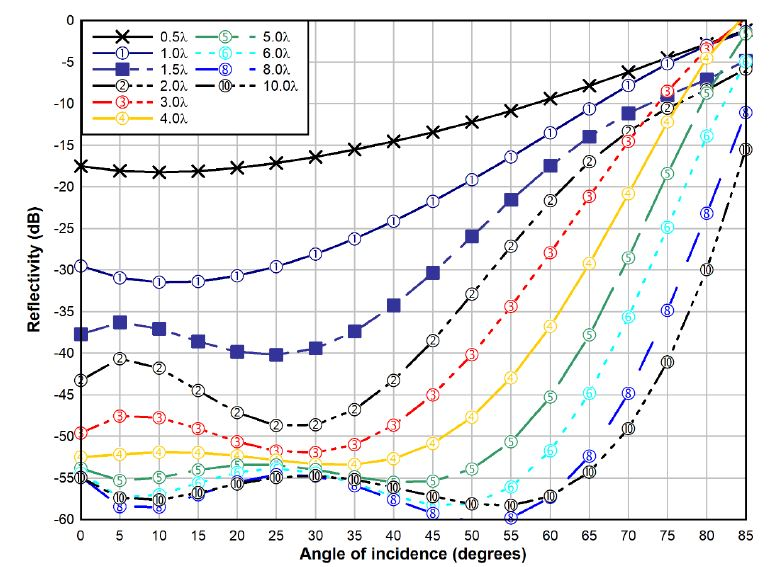
\includegraphics[scale=0.65]{Tabla-limite-angulo-incidencia}
    \caption{Curvas de la relación entre el ángulo de incidencia y la reflectividad}
    \label{Tabla-limite-angulo-incidencia}
\end{figure}

A partir de la gráfica de la figura \ref{Tabla-limite-angulo-incidencia} podemos llegar a una conclusión relativa a la longitud necesaria que debe medir nuestro absorbente. Estableciendo que, con la condición de que el absorbente sea más grande que la longitud de onda, podemos afirmar que el absorbente va a rendir correctamente y no vamos a tener ecos.
\\

Si aplicamos esta idea a un ejemplo práctico para hacernos una idea de lo que supone, significa que si empleamos una frecuencia de 150MHz perteneciente a la banda de la televisión necesitamos un absorbente que mida al menos 2 m de longitud. Estableciendo así la idea de que cuanto menor sea el tamaño de esta pirámide de absorbente, mayor será la frecuencia mínima a partir de la cual podemos efectuar mediciones sin tener efectos difractivos. 

\newpage

\subsection{Límite del tamaño de la cámara}

Al trabajar sobre una cámara anecoica rectangular, no solo debemos tener en cuenta el límite impuesto por el absorbente, sino también la longitud de la cámara. Esto se debe a que la longitud de la cámara nos va a limitar la longitud de onda mínima que podemos usar si queremos medir una antena de tamaño concreto en nuestra cámara y utilizar esas medidas como representativas del campo lejano.\\ 

Bajo esta premisa, urge conocer la distancia a partir de la cual podemos considerar las medidas del campo como medidas del campo lejano, la cual es fácilmente obtenible a partir de la siguiente expresión: 

                            \begin{equation}
                            R =\frac{2D^2}{\lambda}
                            \end{equation}
                       
Donde D es el tamaño de la apertura de nuestra antena y ${\lambda}$ es la longitud de onda en el vacío.\\
Esta expresión se puede reescribir de la siguiente forma si asumimos que el tamaño de la antena será de $n$ veces ${\lambda}$.

                            \begin{equation}
                            R =2n^2\lambda
                            \end{equation}

A partir de estas expresiones podemos obtener cual es la longitud de onda máxima que podemos emplear para medir nuestra antena si conocemos cuanto mide el largo de nuestra cámara anecoica rectangular. Así obtenemos el límite de trabajo de la cámara impuesto por el tamaño de la misma. 

\newpage

\subsection{Estudio de ambos límites combinados}

Una vez presentadas y explicadas ambas limitaciones, es interesante estudiar cómo se combinan entre si, dado que nos van a marcar la frecuencia mínima y máxima que podemos usar en una cámara. 
\\

Para ello, haremos uso de la gráfica vista en la figura \ref{Tabla-limite-angulo-incidencia}, de la cual extraemos el dato de que el absorbente piramidal de altura de $2\lambda$ debe proporcionar una atenuación de 40 dB en la reflexión. 
\\

A partir de esta reflectividad y definiendo $\theta$ como el ángulo de incidencia límite a partir del cual el rendimiento del absorbente decae, podemos obtener la distancia a partir de la cual cumplimos el requisito de campo lejano. Para encontrar dicha condición matemática, debemos aplicar relaciones trigonométricas. Motivo por el cual hemos representado el problema a resolver en la figura \ref{Geometría-del-ángulo-incidencia-absorvente} para facilitar las cosas. 

\begin{figure}[h]
    \centering
    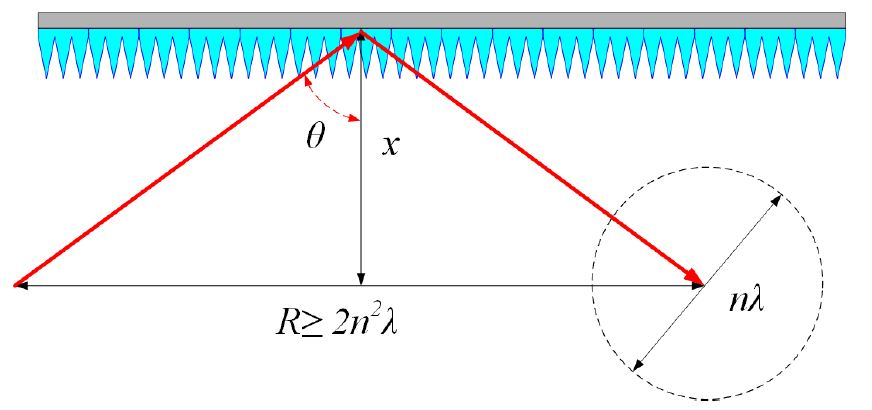
\includegraphics[scale=0.65]{Figura2-Geometria del angulo incidencia}
    \caption{Geometría del ángulo de incidencia en el absorbente de la cámara.}
    \label{Geometría-del-ángulo-incidencia-absorvente}
\end{figure}


Tras una serie de cálculos, somos capaces de obtener la siguiente expresión, que en un principio podría tomar cualquier valor: 

                        \begin{equation}
                        \tan\theta =\frac{R}{2x}
                        \end{equation}

\noindent
donde x es la distancia. 

\newpage

\section{Explicación de la toma de medidas}

Tras haber dedicado una sección a comprender el tipo de instalación que vamos a utilizar y las limitaciones que implica usarla, estamos a disposición de explicar cómo se efectúa la toma de medidas dentro de una instalación.\\

Durante el proceso de medida de una antena interactúan diversos sistemas de forma conjunta para poder caracterizar su comportamiento. La forma de trabajo de estos sistemas y su papel en la toma de medidas nos va a permitir hacernos una idea del proceso que nos permite caracterizar la antena bajo estudio. Debido a esto, esta sección se centra en comprender a alto nivel la arquitectura empleada en una cámara anecoica y cómo sus elementos nos permiten efectuar la toma de medidas .

\subsection{Arquitectura tipica de una cámara anecoica} 

En secciones anteriores hemos hecho referencia a la idea de que no todas las instalaciones son válidas para todos los tipos de antenas debido a que los requisitos necesarios para caracterizar una antena pasiva de un solo puerto son menos exigentes que los necesarios para medir una esfera de antenas de múltiples puertos usada en comunicaciones inalámbricas de alta velocidad. 
\\

Debido a esto y frente a la posibilidad de tener que construir una arquitectura totalmente nueva para cada tipo de antena, se decidió plantear un modelo general que podemos encontrar definido en el estándar 149-2021 \autocite{IEEEstd} y que toma la siguiente forma:

\begin{figure}[h]
    \centering
    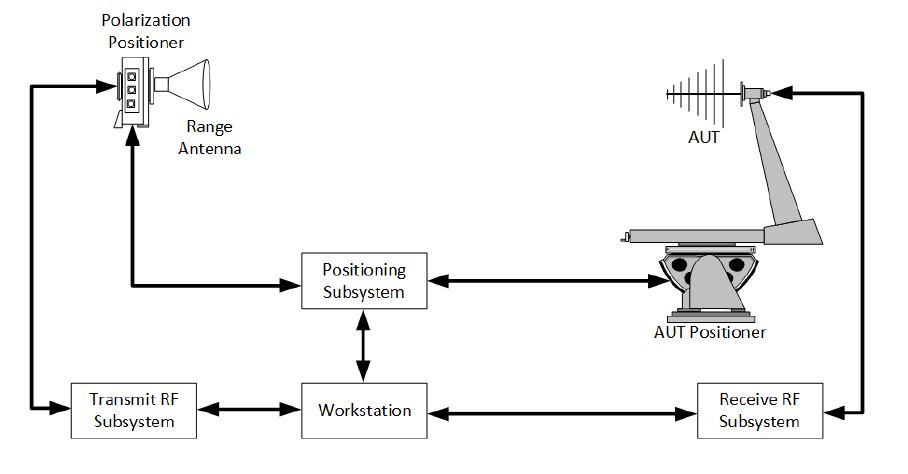
\includegraphics[scale=0.75]{Figura3-Modelo de una estacion completa de medidas}
    \caption{Esquema de una estación de medidas.}
    \label{Modelo-general-de-una-estación-de-medidas}
\end{figure}

\noindent
De todos los elementos presentes en esta arquitectura, nos vamos a centrar en dos de ellos, la antena transmisora y el subsistema de posicionamiento. Esto se debe a que nuestro objetivo no es detallar en profundidad cada subsistema, sino comprender todos los aspectos clave del proceso de medidas que necesitamos saber de cara a comprender las transformaciones.


\subsubsection{Sonda} 

Si nos fijamos en la figura \ref{Modelo-general-de-una-estación-de-medidas}, vemos la aparición de un elemento sobre el que debemos hablar antes de proseguir, la antena transmisora. Hasta ahora únicamente hemos hablado de que, idealmente, para caracterizar el campo lejano de una antena debemos radiar sobre ella una onda plana uniforme y del hecho de que en la realidad usamos ondas semejantes debido a que no es posible generar una onda plana ideal, pero no hemos comentamos nada relacionado con el emisor que usamos para transmitir dicha onda, el cual es precisamente el objeto de estudio de esta sección.
\\

El uso de esta antena transmisora, denominada sonda de ahora en adelante, es necesario para poder transmitir nuestra onda plana a la AUT para poder obtener medidas. Este hecho supone que en aras de poder conocer el comportamiento de la antena bajo test debemos conocer a la perfección el comportamiento de nuestra sonda, ya que de lo contrario no podremos discernir si las medidas son o no coherentes con respecto a lo enviado por la sonda.
\\

Otro concepto a destacar del uso de la sonda, es la idea de que nuestro sistema de medidas se basa en el uso de dos antenas, lo que da lugar a diferentes configuraciones posibles en función de donde se sitúan la sonda y la AUT. Debido a esto, existen diversas configuraciones en función de dónde estén situadas las antenas. Lo que da cámaras donde se pueden intercambiar de posición, otras donde las dos antenas están combinadas en un mismo instrumento y otras en las que ambas antenas están en posiciones fijas como la ilustrada en la figura \ref{Modelo-general-de-una-estación-de-medidas}. Pese a esto, independientemente de la configuración ante la que estemos, el funcionamiento de cada sistema es idéntico, por lo que todo lo visto a continuación es válido independientemente de dónde estén situadas las antenas. 

\subsubsection{Frecuencia de trabajo}

A excepción de algunas instalaciones especializadas en ciertos tipos de medida, es habitual que las instalaciones de medida se diseñen para usar un rango de frecuencia lo más amplio posible que cumpla los límites aceptables de funcionamiento presentados en secciones anteriores.\\

Pese a lo anterior, operar sobre un rango amplio de frecuencia trae consigo un problema principal relacionado con que usualmente el rango de frecuencias deseado excede el ancho de banda de trabajo de nuestra sonda. Razón por la cual es habitual disponer de una familia de antenas que en conjunto si permitan cubrir dicho rango de frecuencias. Este hecho implica la necesidad de disponer de un grupo de antenas que presenten una ganancia, ancho de haz y polarización coherentes con las medidas que queremos realizar nuestro rango, ya que no todas las antenas disponen de los mismos requisitos de línea de visión, reflexión o rangos compactos.\\

Otro aspecto a tener en cuenta es que necesitamos caracterizar la AUT en ambas polarizaciones, horizontal y vertical, lo que implica que necesitamos una forma de poder controlar la polarización usada en nuestra sonda. Empleándose usualmente sondas polarizadas de forma ortogonal o montando una sonda de polarización lineal sobre un posicionador de polarización que permita orientar el ángulo de inclinación de la polarización.


\subsubsection{Subsistema de posicionamiento} 

Para poder caracterizar una antena necesitamos tomar medidas del campo para los todos los ángulos de trabajo significativos, lo cual es posible gracias al subsistema de posicionamiento encargado de controlar la orientación de la sonda y la AUT durante el proceso de medida. Debido al hecho de que vamos a estar tratando con posiciones en el espacio, debemos apoyarnos en un sistema de coordenadas que nos permita asociar las medidas con la posición de las antenas, el cual típicamente es el sistema de coordenadas esférico. Al trabajar sobre este sistema de coordenadas, independientemente de si la línea de visión es fijas o móvil, dispondremos de dos ejes ortogonales que combinados permitan efectuar cortes en $\theta$ y $\phi$. Estos ejes se designan como el eje de rotación $\theta$ y el eje de rotación $\phi$. Los cuales están representados en la siguiente figura. 

\begin{figure}[h]
    \centering
    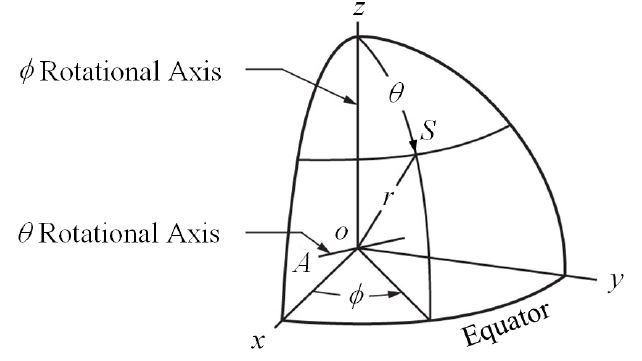
\includegraphics[scale=0.65]{Figura6-Ejes ortogonales para medir antenas}
    \caption{Ejes de rotación en un sistema esférico.}
    \label{Ejes-ortogonales-para-medir-antenas}
\end{figure} 

\noindent
En nuestro caso particular, la sonda está fija y haremos pivotar la AUT de forma que podamos tomar medidas en un rango significativo de ángulos.